
\chapter{Research Results}
\section{Overview} 
This chapter has my analysis of my participants usage of the Steam service during the Concurrent Think-Aloud study. This analysis includes the following data metrics; Errors and issues encountered, Task Duration, Task Completion and Task Mouse Interactions, spilt between the Novice and Experienced groups. Kruskal-Wallis tests were used to assess the difference between Novice and Experienced participants with the four metrics. These Kruskal-Wallis tests have been calculated at the 95\% confidence interval, therefore results that equal 0.05 or less mean that there is a significant difference and the null hypothesis is rejected that there is no difference.  


\section{Error and Issue Detection}
The following section details all notable errors and issues that were encountered by both sets of participants during this UX study. This is followed by the most common issues that were encountered by both experience groups. Issues refer to a problem caused by the user directly, whereas errors are were the service behaves unexpectedly. An example of an issue, is navigating to the wrong part of the service when attempting a task, such as clicking upon the wrong Workshop for Task C. An example of an error could be something like a black screen, or a \gls{ui} such as flickering or images and text not being scaled correctly. Issues were the most common type of problem encountered, and very few errors were experienced by either novices or experienced participants. Therefore as such Steam is a well built system, but it does have some frustrating elements which newer users will encounter and could be described as somewhat convoluted. Additionally I have also conducted a Kruskal-Wallis test to determine any significance difference between Novice and Experienced participants regarding the number of issues and errors encountered during their usage of the Steam service. This has been conducted with each task, issues in multiple tasks,generic issues and all issues per participant.

\subsection{Novice Participant Error and Issues}
\begin{table}[H]
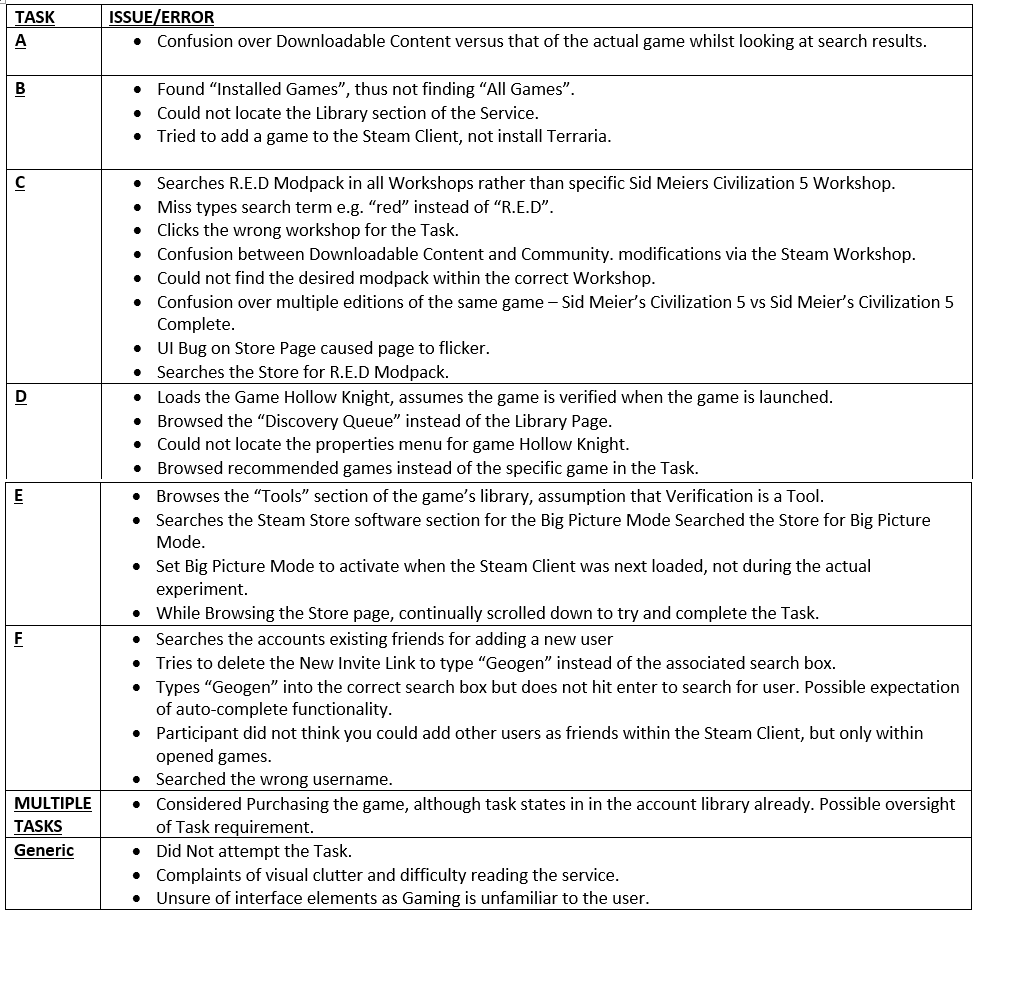
\includegraphics[width=\linewidth]{Screenshots/ErrorRecords/Novice/noviceAllErrors.png}
\label{NoviceErrorsList}
\caption{All Novice Issues and Errors Detected}
\end{table}

Table 5.1 shows all issues and errors that were encountered by my Novice participants during there use of the Steam program. In total there were 30 unique issues encountered which has been presented within the table. However there were variations upon these errors but they were too similar to deem them as a separate error and as such are not present within this table. It is clear that Task C proved the most challenging for the Novice sample with a total of eight out of 29 issues, accounting for 27.5\% of all issues. This was somewhat expected as was stated in Chapter 3, Task C was deliberately more complex task, and as there was the expectation of more issues than other tasks.  Surprisingly Task F had several a total of five unique errors despite the relative similarity to other more commonly used services such as social media, as the task was to add another user as a friend, much like on those other platforms.

\begin{figure}[H]
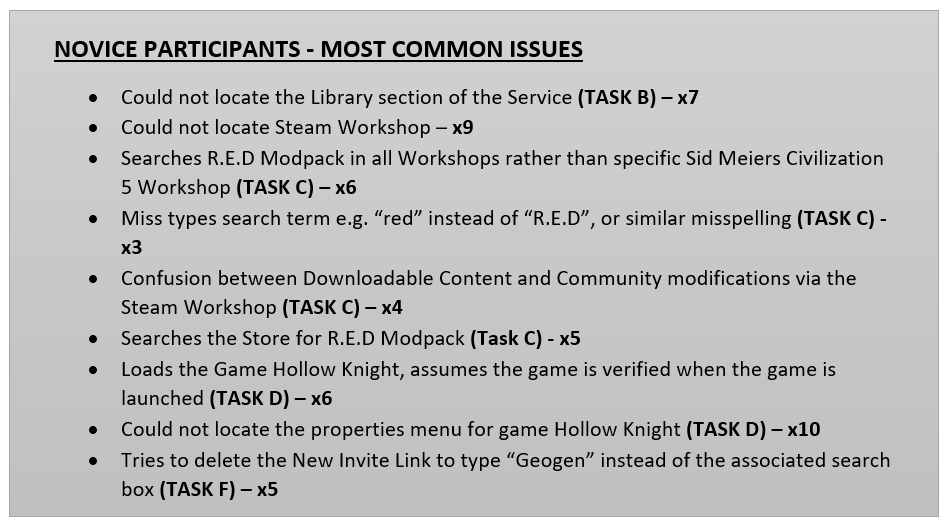
\includegraphics[width=\linewidth]{Screenshots/ErrorRecords/Novice/noviceMostCommonIssues.png}
\label{NoviceMostCommonErrors}
\caption{Most Common Issues encountered by Novice Participants}
\end{figure}

The issues displayed in Figure 5.1 show that the most common issue was in relation to Task D, the verification of a games files and being unable to locate the correct interface element to initiate this process. The prevalence of this issue is not entirely unexpected, as Novice users are less familiar with gaming themes, the word ``verification" is in part the reasoning for why this particular task proved difficult. However this issue has highlighted an issue with the Steam client in how this functionality is shown within the Steam client. A user must know that they have to right click upon the desired game to display the games properties menu, 10 participants failed task D because of this reason as this function is not at all obvious for a new user. Task D is also interesting due to the existence of another issue, that is six novices loaded the game ``Hollow Knight" as they believed that the Task was a trick question and that verification was irrelevant. Therefore the inclusion of this task has highlighted to me that the selection of tasks, and the wording of the task influence generation of issues as well as the service tested itself.

Task C also had three very common issues, which are all directly related to one another as they regard the search functionality of the Steam client. Task C asked users to find a modification for Sid Meier's Civilization 5, which is found within the Steam Workshop functionality. Most users attempted this task in a logical way, by searching for the desired modification, however where the participant searched provided to be problematic for several novice users, by entering ``R.E.D modpack". However several users entered this search term into the search for all game workshops and therefore did not find the desired subscribe tool as the task required. Five other novices decided that they would try to search for the modpack within the steam store page, thus returning products to buy with the word ``red" within them, and therefore irrelevant results for the task. 

Task F's main issue was partially a layout issue as five Novices did not see the search functionality for adding fellow users by name, in the test case ``Geogen". Instead Novices were drawn to using the \gls{nil}. The intended purpose of NIL is to send a link to the desired user by email or SMS, thus requiring an external device in order to connect two users together. Once a link is generated it can only be shared or deleted. Five users however decided to try to type the desired user name of ``Geogen" into the NIL but were unable to do so, and thus became puzzled at the lack of functionality and thus become unable to complete the task correctly.

\subsection{Experienced Participant Error and Issues}

\begin{table}[H]
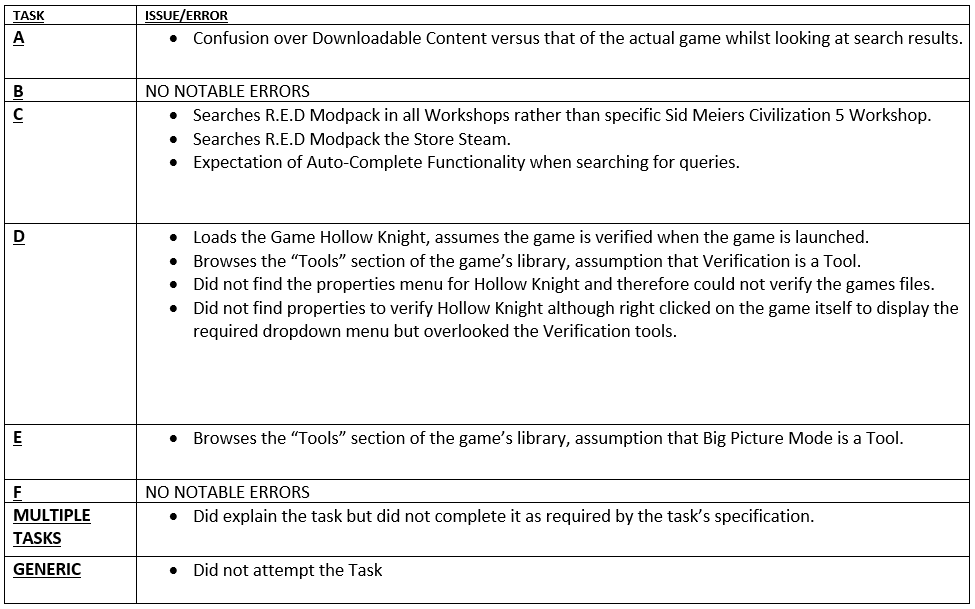
\includegraphics[width=\linewidth]{Screenshots/ErrorRecords/Experienced/experiencedAllErrors.png}
\label{ExperiencedErrorsList}
\caption{All Experienced Issues and Errors Detected}
\end{table}

Table 5.2 is the Experienced total issues and errors encountered during the study. In total there were fewer issues and errors encountered compared to that of the novice participants with a total of 11 overall unique issues. Similarly to that of the Novice participants however, was the presence of issues in Task C , with identical issues being encountered by some of the participants. Another notable aspect is that Task B and task F had no notable issues with the Experienced participants with all participants successfully completing these tasks. Fewer generic issues were also detected by Experienced Participants. 

\begin{figure}[H]
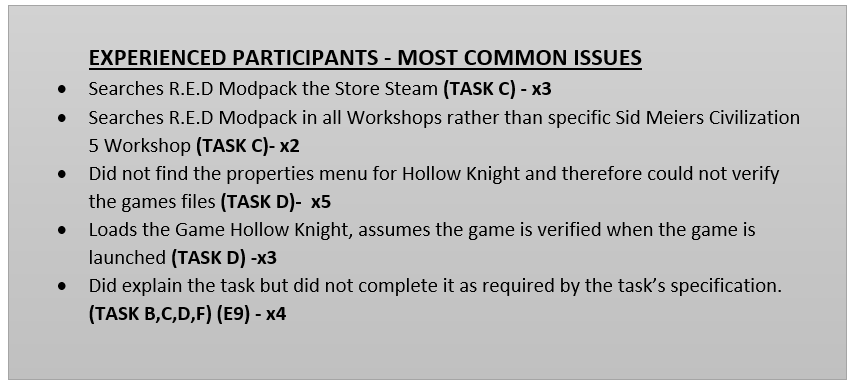
\includegraphics[width=\linewidth]{Screenshots/ErrorRecords/Experienced/experiencedCommonErrors.png}
\label{ExperiencedMostCommonErrors}
\caption{Most Common Issues encountered by Experienced Participants}
\end{figure}

This figure shows the most common issues that were encountered during the Novice testing session. Task D had the most common issue, as five participants out of 16 were unable to locate the properties menu needed to access the verification tools. This issue was very common in the experienced category as well, and therefore shows that Novice and Experienced participants do encounter similar issues during this particular study. Task C also had the same type of issues encountered by Novice participants, whilst trying to find the R.E.D Modpack and using the wrong searching tools. The most notable other type of issue was in the case of one participant (Participant E9) who when asked to complete the tasks they explained how they were going to use the program in order to complete the task, but did not then proceed to complete the tasks in the the manner they described, this behaviour was exhibited during Tasks B,C,D and F but not Task A or E. Although the way in which participant E9 explained their indented use of would have caused them to complete the tasks correctly, they way in which they responded highlights the importance of how the Tasks are explained to the participant, and thus the role of the practitioner cannot be understated during similar Concurrent Think-Aloud studies.

\subsection{Error Type Summary}
It can be summarised that based on this data, the types of errors encountered are broadly similar in both experience categories. There are some exceptions to this, with Experienced participants finding no specific issues with Task B or Task F. However experienced participants did display more issues regarding multiple tasks.

\subsection{Number of Errors By Experience Group}
\begin{table}[H]
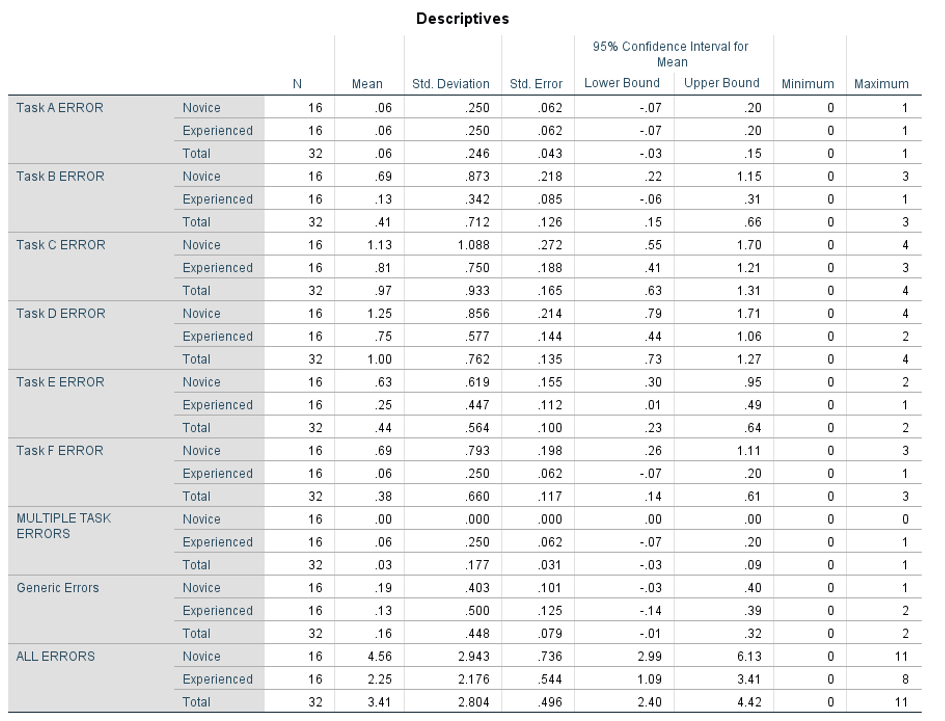
\includegraphics[width=\linewidth]{Screenshots/ErrorRecords/errorBreakdownDescriptives.png}
\label{DescriptivesErrorsPerGroup}
\caption{Descriptive Statistics for Number of Issues Encountered by Experience Group}
\end{table}

Table 5.3 shows descriptive statistics taken from both the Novice and Experienced participant groups regarding the number of errors encountered per group type. All samples were used during this analysis with 16 participants within each group. Task C and D show the highest average mean issues detected within the Novice category, with 1.13 and 1.25 errors detected per participant on average for Task C and D respectively. This trend continues with Experienced Participants with 0.81 and 0.75 issues detected for Task C and D respectively. As anticipated Novices had a higher frequency of errors overall compared to that Experienced Participants, with 4.56 issues discovered by Novices versus that of only 2.25 issues found by Experienced participants on Average, although the highest number of issues detected was 11 for a Novice participant and 8 for an experienced. Attention should be paid to the results regarding the lower bounds of several tasks, as some of these results return negative values, these values should be ignored and considered as zero. This is due to the fact that participants cannot encounter a negative amount of issues during their usage of Steam or other tested services in usability testing.

\begin{table}[H]
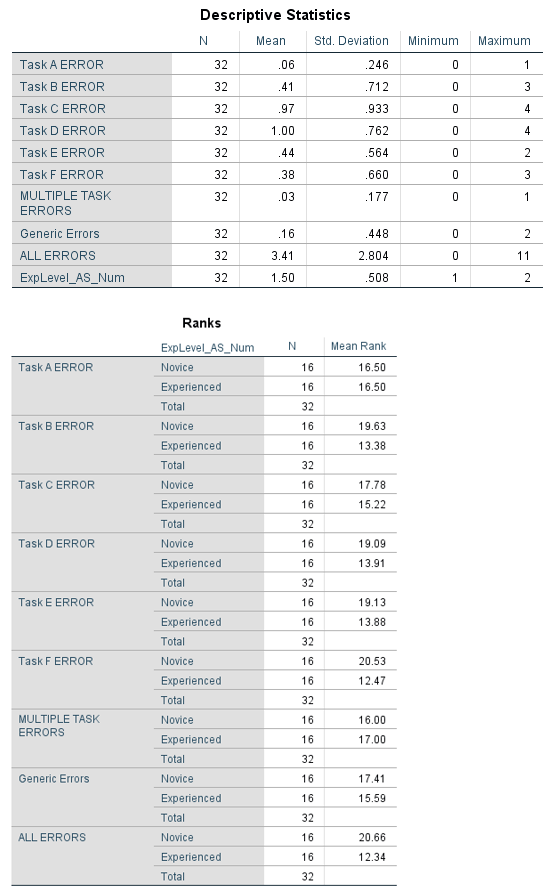
\includegraphics[width=\linewidth]{Screenshots/ErrorRecords/kwDescriptiveErrors.png}
\label{KWErrorsPerGroup}
\caption{Kruskal-Wallis Examination for Number of Issues Encountered by Experience Group}
\end{table}

Table 5.4 shows a condensed version of Table 5.3 with all participant data combined in a Task by Task format, retaining core descriptive statistics. However the second table shows the Mean rank distribution of errors encountered by participants on an experience level basis. As can been seen within this table, the majority of the results show a higher Mean rank for Novice participants in all categories with the exception of  Task A and Multiple Task Errors. Task A shows an equal Mean rank as only one type of error was encountered during this study between the two groups. The Mean rank of multiple task errors can be explained by the results of participant E9 which was explained in Figure 5.2. These results partially answer one of my research questions (RQX2), as it shows that more errors are detected by Novice participants than Experienced ones with regards to the entire sample population of each category.

\begin{figure}[H]
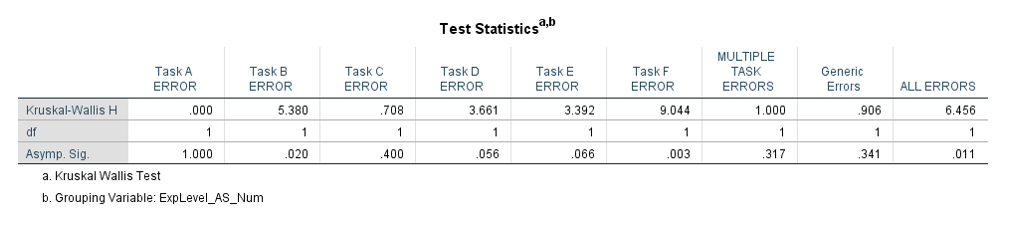
\includegraphics[width=\linewidth,height=6cm]{Screenshots/ErrorRecords/kwErrorsByParticipant.png}
\label{KWErrorsPerGroup}
\caption{Kruskal-Wallis Examination for Number of Issues Encountered by Experience Group}
\end{figure}

Figure 5.3 are the results of a Kruskal-Wallis examination with the numbers of errors detected between Novice and Experienced participants, as calculated at a 95\% interval. On a Task by Task basis, there is no significant difference in Novice and Experienced participants regarding the number of errors detected. This is with the exception of Task F, which shows a Assumption figure of 0.03.  Interestingly, the result for the All errors category also shows that there is no significant difference between the two experience groups, although it is close to the threshold of 0.05 compared with all other Task results. Therefore, it Novice and Experienced participants are not significantly different in regard to the number of individual issues and errors experienced on a per participant basis. However, as shown by the Table 5.4 more errors were detected by the Novice sample population overall compared with the Experienced sample population. 

\section{Task Duration}
The following section details collected data from participants in regards to each tasks duration. Each task's data had a Kruskal-Wallis test performed between Novice and Experienced data sets to ascertain if there was any significant difference between the two groups. Two sets of descriptive data also accompany these results, as to show various variations between the data sets.

\begin{table}[H]
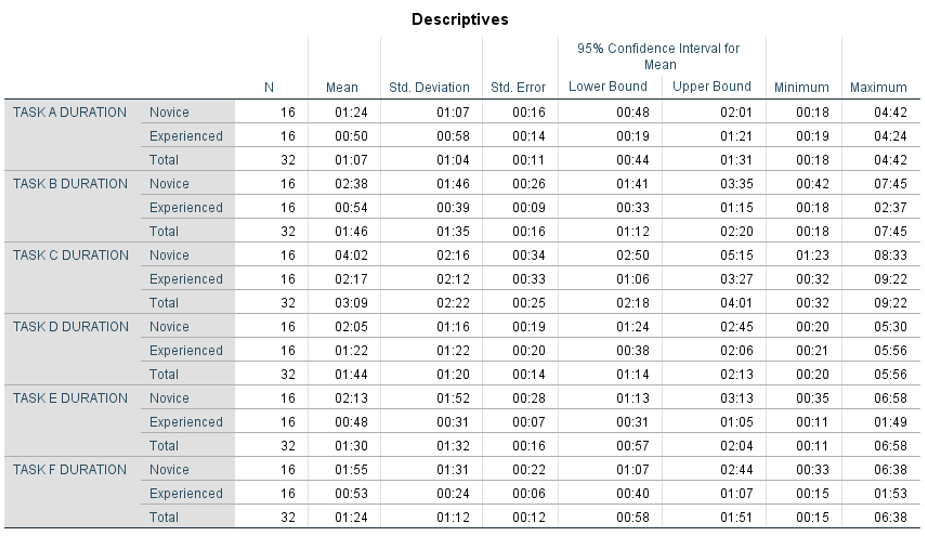
\includegraphics[width=\linewidth]{Screenshots/UXResearchDataFiles/UXTaskDurationData/anovaDescriptivesTaskDuration.png}
\label{DurationOverallStats}
\caption{Task Duration - Descriptive Statistics Novices and Experienced Participants}
\end{table}

This table displays several useful descriptive statistics, including the Mean, Standard Deviation,Standard Error, Minimum value and Maximum values. Critically this data set displays the upper and lower bounds of the data set to a confidence interval of 95\%, for both Novice and Experienced participants and for all tasks attempted. It should also be noted that all tasks data was included, therefore totalling 32 pieces of data per task and 192 pieces of data overall, whilst assessing Task Duration. The longest average time spent on one particular Task for Novice participants was Task C with one participant taking 08:33 minutes to attempt the Task, of further interest is the longest Experienced participant time for one task, which was also Task C taking 09:22 minutes to complete which is surprising. However the majority of these statistics describe a trend that I had expected, that Novice participants took longer to attempt the same tasks as Experienced participants. Task C still proved to be the longest Task on average for both Novice and Experienced participants, which I anticipated as Task C was the most difficult task to complete.  

\begin{table}[H]
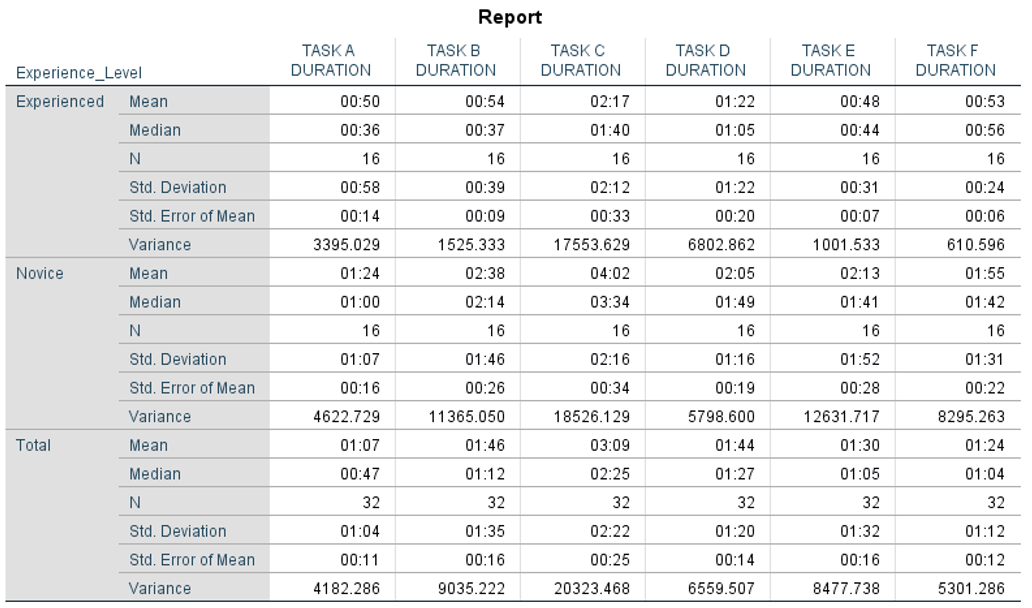
\includegraphics[width=\linewidth]{Screenshots/UXResearchDataFiles/UXTaskDurationData/taskDurationOverallEdited.png}
\label{DurationOverallFurtherStats}
\caption{Task Duration - Further Descriptive Statistics Novices and Experienced Participants}
\end{table}

Further to Table 5.5 this descriptive table shows the variance in the data sets. It should be noted that all Experienced participant Task Duration's data sets have less variance between each participants results with the exception of Task D which shows greater variance compared to that of Novice participants. Therefore with the exception of Task D, these results show a greater variance in the time it took Novice participants to attempt or complete each Task. The greatest variance in results for both Novice and Experienced groups was Task C, this is especially prominent when both sets of data are collected into one, which links with the descriptive data as detailed above in Table 5.5. It should also be noted that the biggest difference in variance between Novice and Experienced participants is seen in the results for Task F followed closely by Task E.Task F Experienced participants data sets scored a variance of 610.6, whilst the Novice participants data scored 8295.3 a percentage increase of 1258.55\%. Task E Experienced participants had a variance score of 1001.533, whereas the Novice data set shows a score of 12631.717, a percentage increase of 1161.24\%. Task B also shows a major difference in variance between the two participant types. Therefore it is clear that these data sets vary regarding these Tasks, but show similarity with Tasks A,C and D.

%\begin{table}[H]
%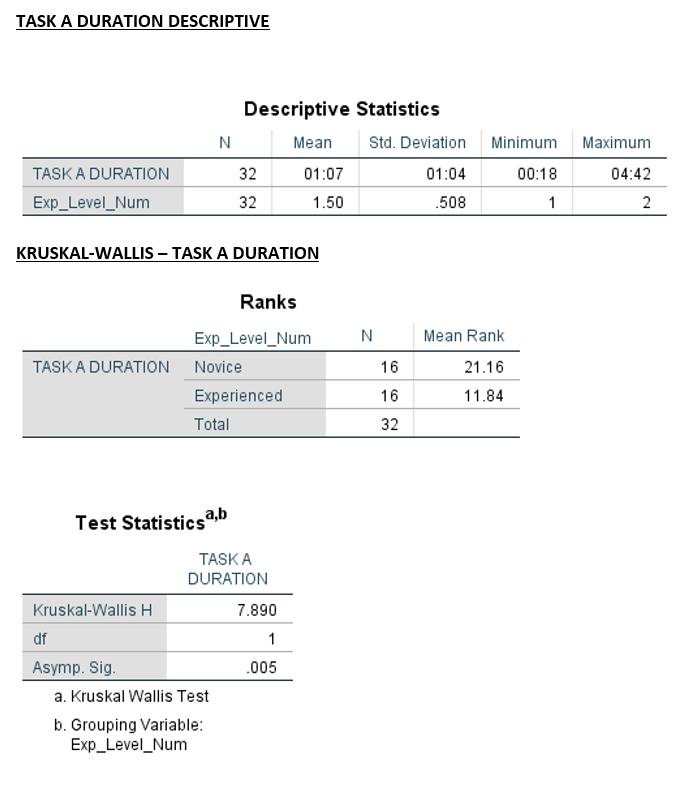
\includegraphics[width=\linewidth]{Screenshots/UXResearchDataFiles/UXTaskDurationData/taskDurationAStatsEdited.png}
%\label{DurationTaskA}
%\caption{Task A Duration Results}
%\end{table}

%\begin{table}[H]
%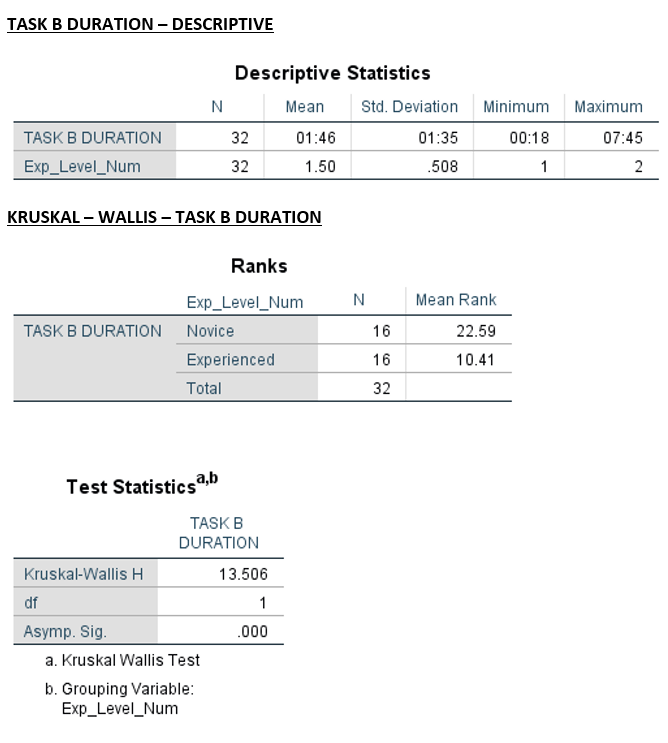
\includegraphics[width=\linewidth]{Screenshots/UXResearchDataFiles/UXTaskDurationData/taskDurationBStatsEdited.png}
%\label{DurationTaskB}
%\caption{Task B Duration Results}
%\end{table}

%\begin{table}[H]
%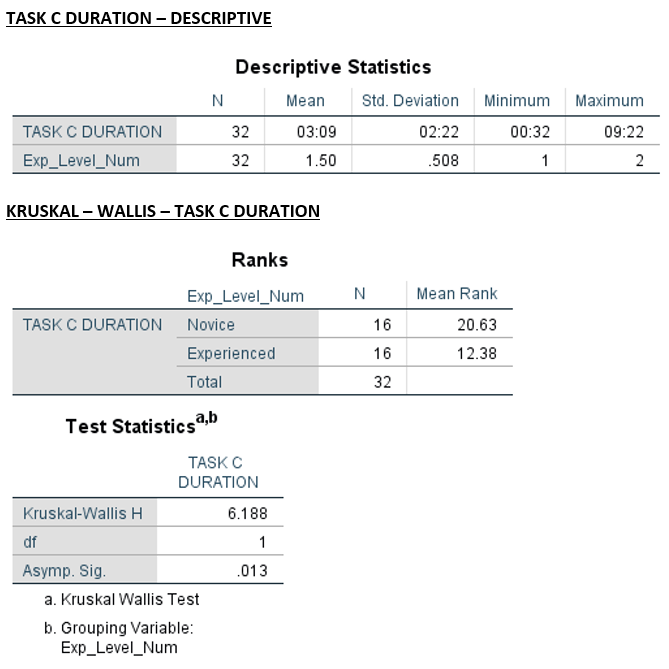
\includegraphics[width=\linewidth]{Screenshots/UXResearchDataFiles/UXTaskDurationData/taskDurationCStatsEdited.png}
%\label{DurationTaskC}
%\caption{Task C Duration Results}
%\end{table}

%\begin{table}[H]
%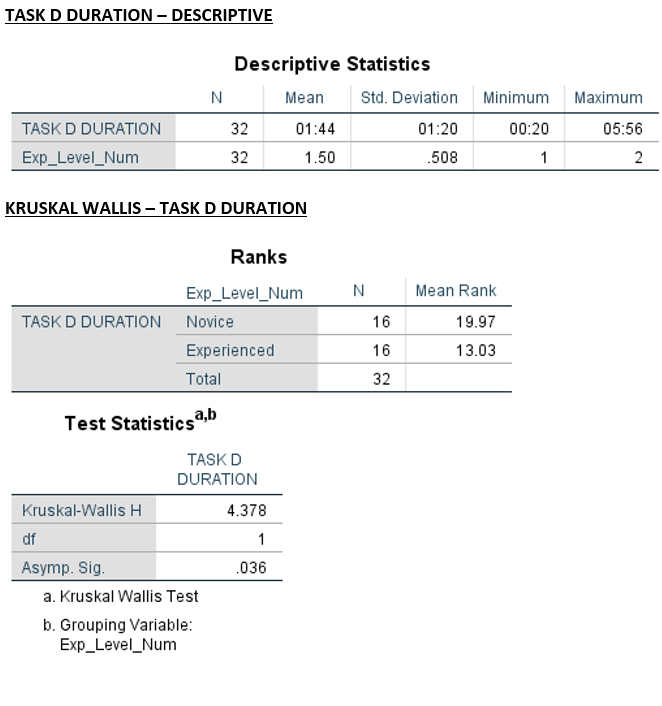
\includegraphics[width=\linewidth]{Screenshots/UXResearchDataFiles/UXTaskDurationData/taskDurationDStatsEdited.png}
%\label{DurationTaskD}
%\caption{Task D Duration Results}
%\end{table}

%\begin{table}[H]
%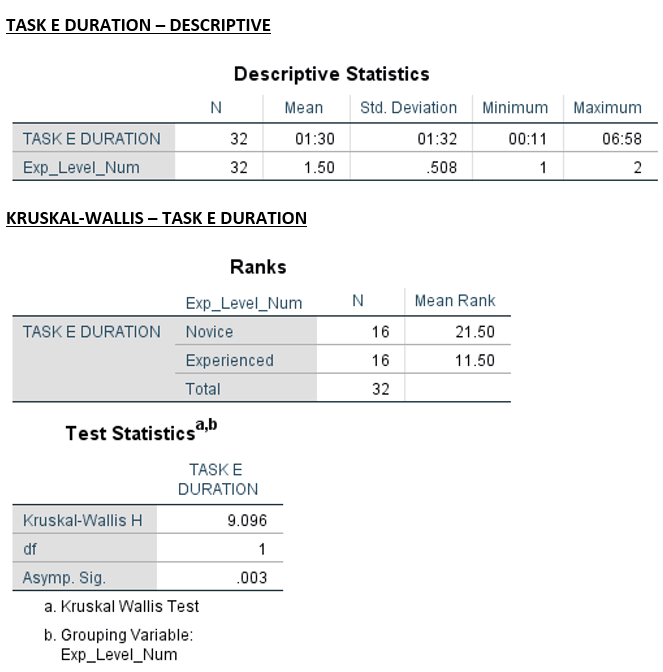
\includegraphics[width=\linewidth]{Screenshots/UXResearchDataFiles/UXTaskDurationData/taskDurationEStatsEdited.png}
%\label{DurationTaskE}
%\caption{Task E Duration Results}
%\end{table}

%\begin{table}[H]
%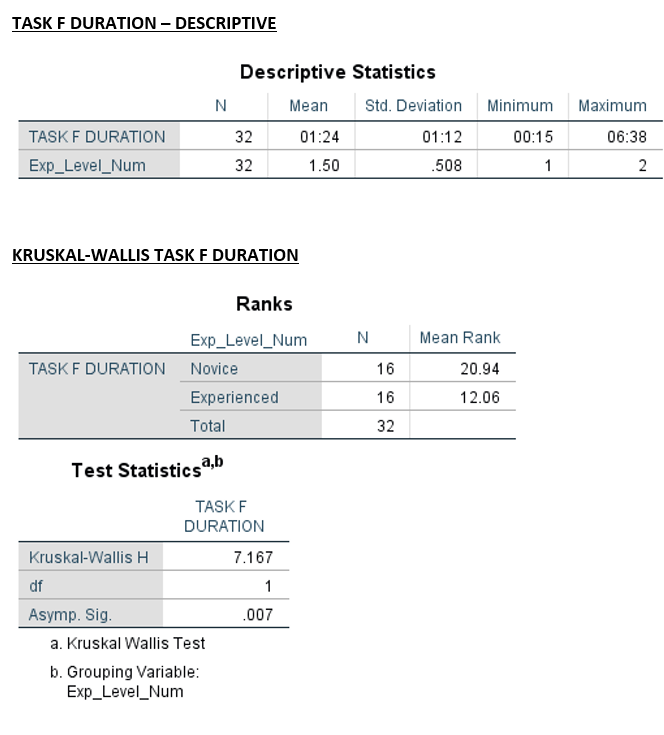
\includegraphics[width=\linewidth]{Screenshots/UXResearchDataFiles/UXTaskDurationData/taskDurationFStatsEdited.png}
%\label{DurationTaskF}
%\caption{Task F Duration Results}
%\end{table}

%\begin{table}[H]
%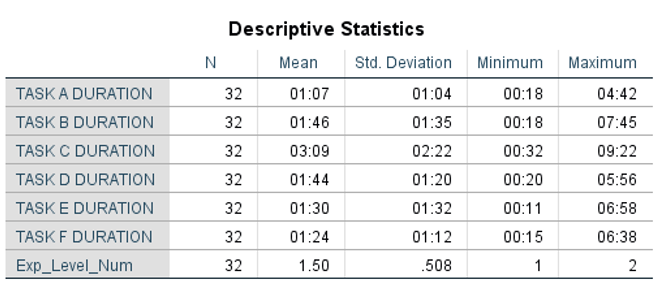
\includegraphics[width=\linewidth]{Screenshots/UXResearchDataFiles/UXTaskDurationData/taskDurationOverallStatsDescriptiveEdited.png}
%\label{DescriptiveDurationTotalPopulation}
%\caption{Task Duration Descriptive Statistics for Total Population}
%\end{table}

\begin{table}[H]
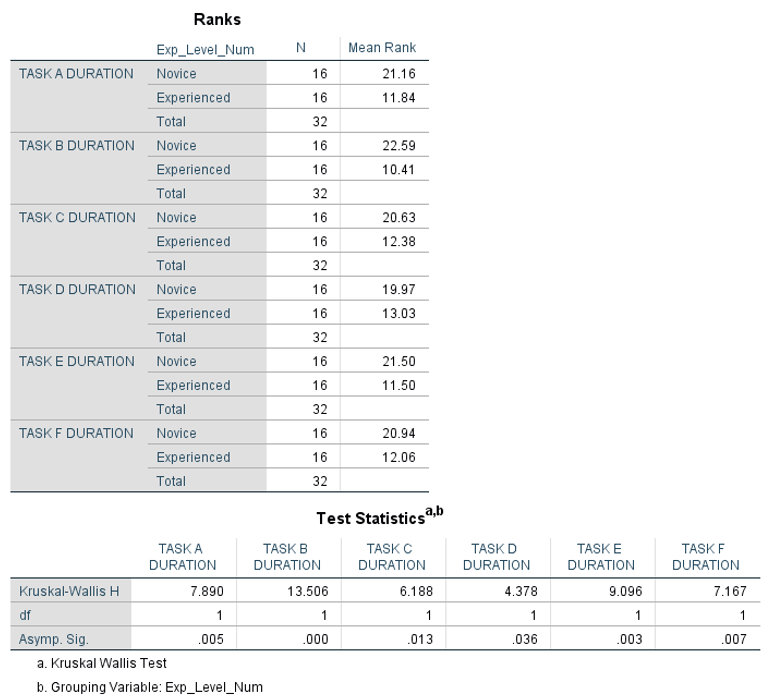
\includegraphics[width=\linewidth]{Screenshots/UXResearchDataFiles/UXTaskDurationData/taskDurationOverallStatsKWEdited.png}
\label{DescriptiveDurationTotalKW}
\caption{Task Duration Descriptive Statistics for Total Population}
\end{table}

This table shows all Task Duration data into one table, including the Mean rank that Novice and Experienced data sets hold, and more interestingly the Kruskal-Wallis examinations per task. Any task with an assumption signature equalling 0.05 or below indicates a significant difference between Novice and Experienced participants in the study. Much like with the participants encountering errors, the Novices have a higher Mean rank, thus demonstrating a greater amount of time spent in each Task compared to that of the Experienced participants. Regarding the Kruskal-Wallis assumption figures it is clear that Tasks A, B and E have the presence of significant differences between that of Novice and Experienced Users, especially with regards to Task B. Thus, Task C, D and F have no significant difference between those of Novice and the Experienced group. Task D shows the most similarity between the two types of user, with a assumption signature of 0.36, which corresponds to the proceed variance results, followed by Task C and F, although Task F almost reaches the threshold needed to be deemed significantly different. Therefore participants of both types interacted with Task C and D in a similar way in terms of how long they spent on each Task as well as Task F.


\section{Task Completion}
\begin{table}[H]
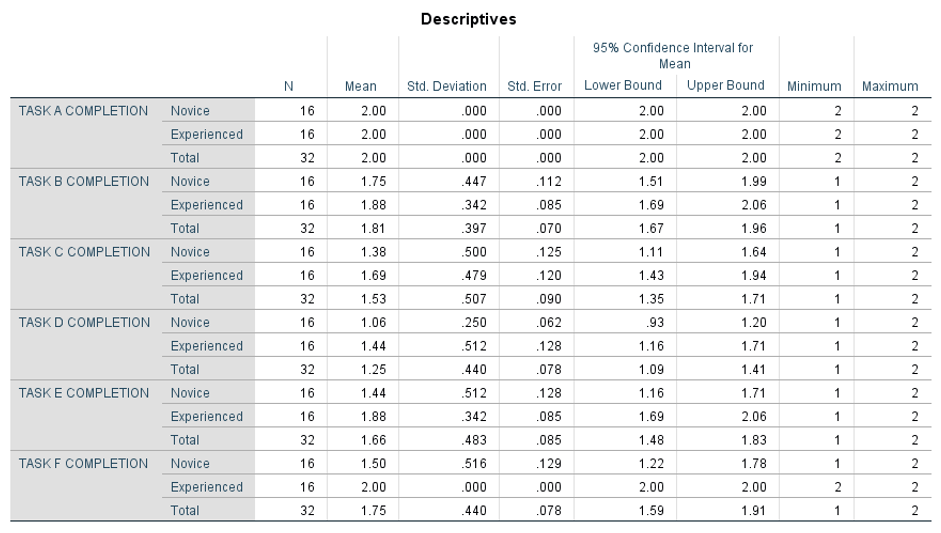
\includegraphics[width=\linewidth]{Screenshots/UXResearchDataFiles/UXTaskCompletionData/anovaDescriptivesTaskCompletion.png}
\label{DescriptiveTaskCompletionTotalPopulation}
\caption{Task Completion - Descriptive Statistics Novices and Experienced Participants}
\end{table}

As with Task Duration, Table 5.8 demonstrates several descriptive statistics analysed from both Novice and Experienced Participants. To determine whether a participant had completed a Task successfully or not, a scoring system was implemented. If a participant scored ``1" the Task was not completed successfully, whilst a score of ``2" meant that the participant completed the Task successfully, that is with the expected outcome. Task A was the only task to be successfully completed by participants of both categories with no participant failing to complete this Task, additionally all experienced participants successfully completed Task F, whereas several Novices were unable to do so. All other Tasks are more varied, but the generic trend showed that Novice participants were unable to complete more tasks compared with the Experienced participants. More detailed figures can be seen within Appendix A, Further Results.

%\begin{table}[H]
%includegraphics[width=\linewidth]{Screenshots/UXResearchDataFiles/UXTaskCompletionData/TaskACOMPLETIONEdited.png}
%\label{TaskCompletionA}
%\caption{Task A Completion Results}
%\end{table}

%\begin{table}[H]
%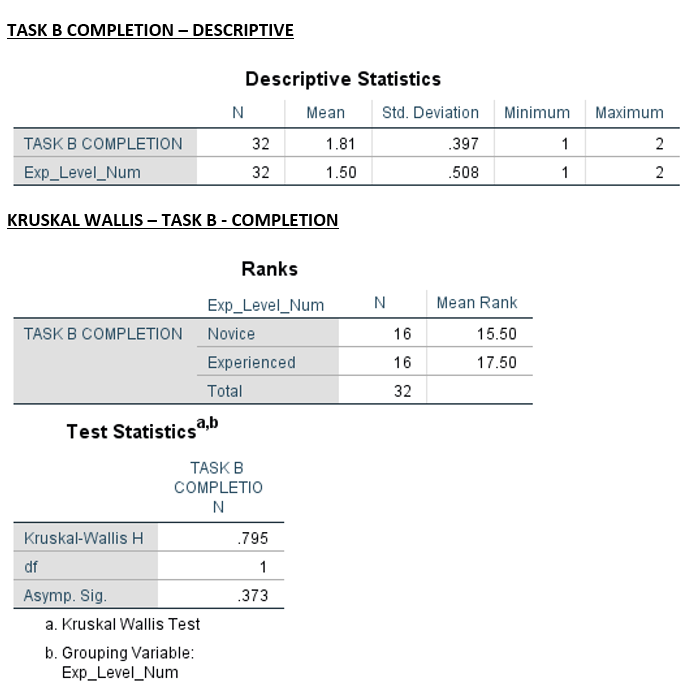
\includegraphics[width=\linewidth]{Screenshots/UXResearchDataFiles/UXTaskCompletionData/TaskBCOMPLETIONEdited.png}
%\label{TaskCompletionB}
%\caption{Task B Completion Results}
%\end{table}

%\begin{table}[H]
%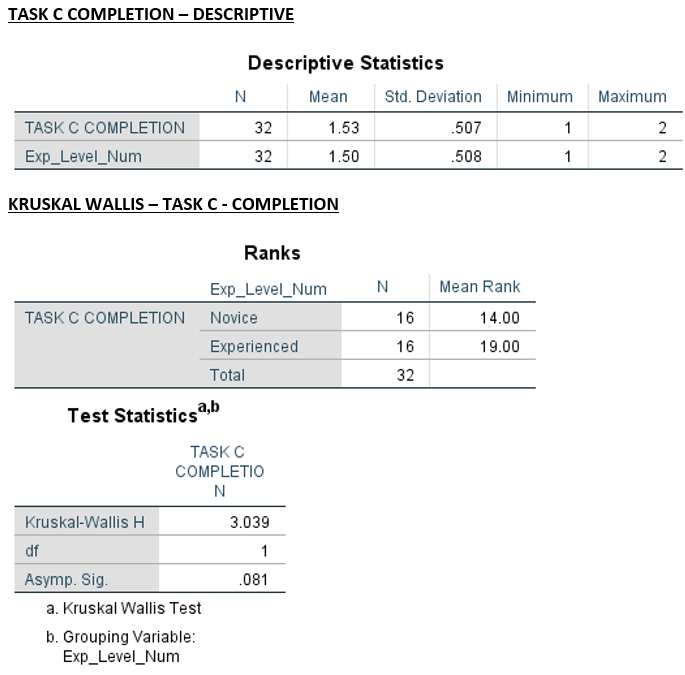
\includegraphics[width=\linewidth]{Screenshots/UXResearchDataFiles/UXTaskCompletionData/TaskCCOMPLETIONEdited.png}
%\label{TaskCompletionC}
%\caption{Task C Completion Results}
%\end{table}

%\begin{table}[H]
%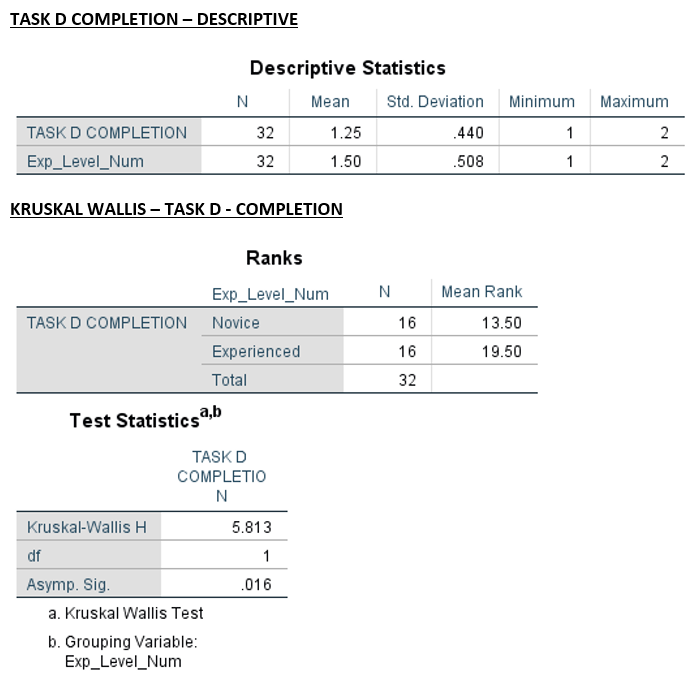
\includegraphics[width=\linewidth]{Screenshots/UXResearchDataFiles/UXTaskCompletionData/TaskDCOMPELTIONEdited.png}
%\label{TaskCompletionD}
%\caption{Task D Completion Results}
%\end{table}

%\begin{table}[H]
%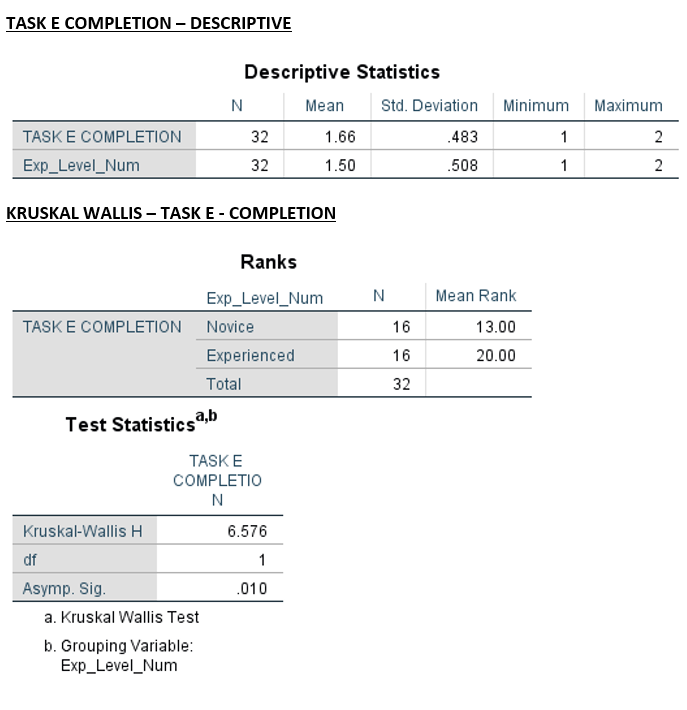
\includegraphics[width=\linewidth]{Screenshots/UXResearchDataFiles/UXTaskCompletionData/TaskECOMPLETIONEdited.png}
%\label{TaskCompletionE}
%\caption{Task E Completion Results}
%\end{table}

%\begin{table}[H]
%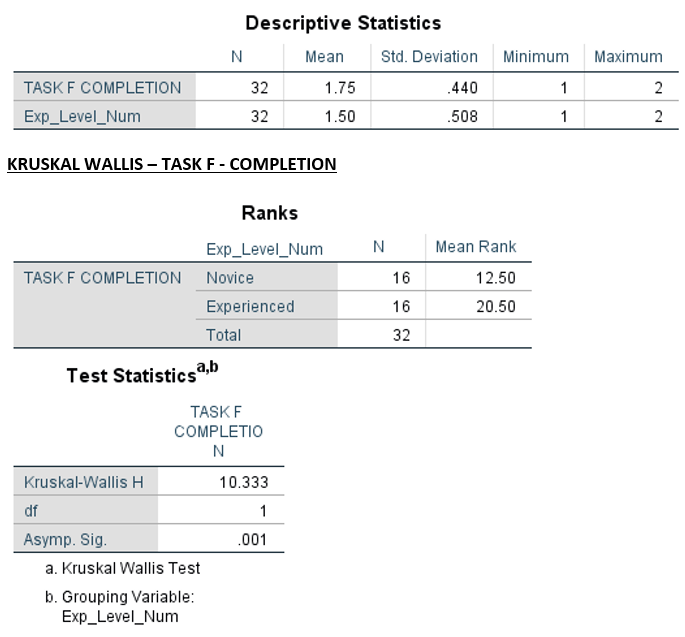
\includegraphics[width=\linewidth]{Screenshots/UXResearchDataFiles/UXTaskCompletionData/TaskFCOMPLETIONEdited.png}
%\label{TaskCompletionF}
%\caption{Task F Completion Results}
%\end{table}

\begin{table}[H]
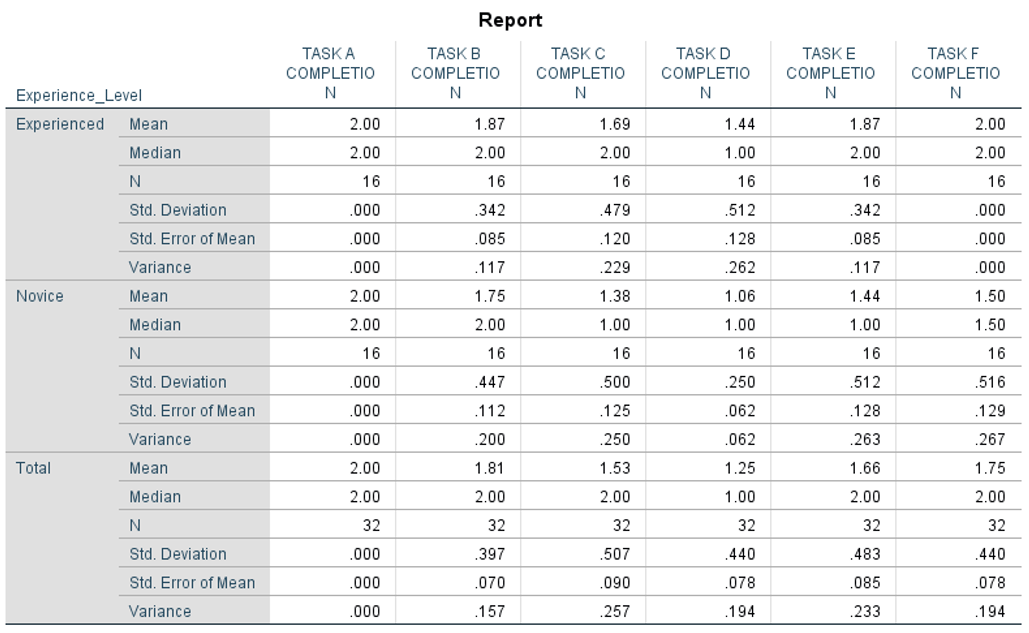
\includegraphics[width=\linewidth]{Screenshots/UXResearchDataFiles/UXTaskCompletionData/TaskCOMPLETIONOVERALLDESCRIPTIVEEdited.png}
\label{DescriptiveTaskCompletionAllTasks}
\caption{Task Completion - Further Descriptive Statistics for Total Population}
\end{table}

Novice and Experienced participants data sets show some variation, with the exception of the aforementioned Task A, where no differences were present between Novice and Experienced users. Task F showed the most variance in the Novice data set, with 50\% of participants completing the task successfully and the remaining failing to do so. Experienced participants show the most variance with Task D, with 43.8\% (7) of experienced participants completing the Task, with the remainder of 56.3\% (9) failing the task. Combining both data sets Task C showed the most variation, with 46.9\% (15) failing and 53.1\% (17) succeeding in completing the Task across both experience groups. 


\begin{table}[H]
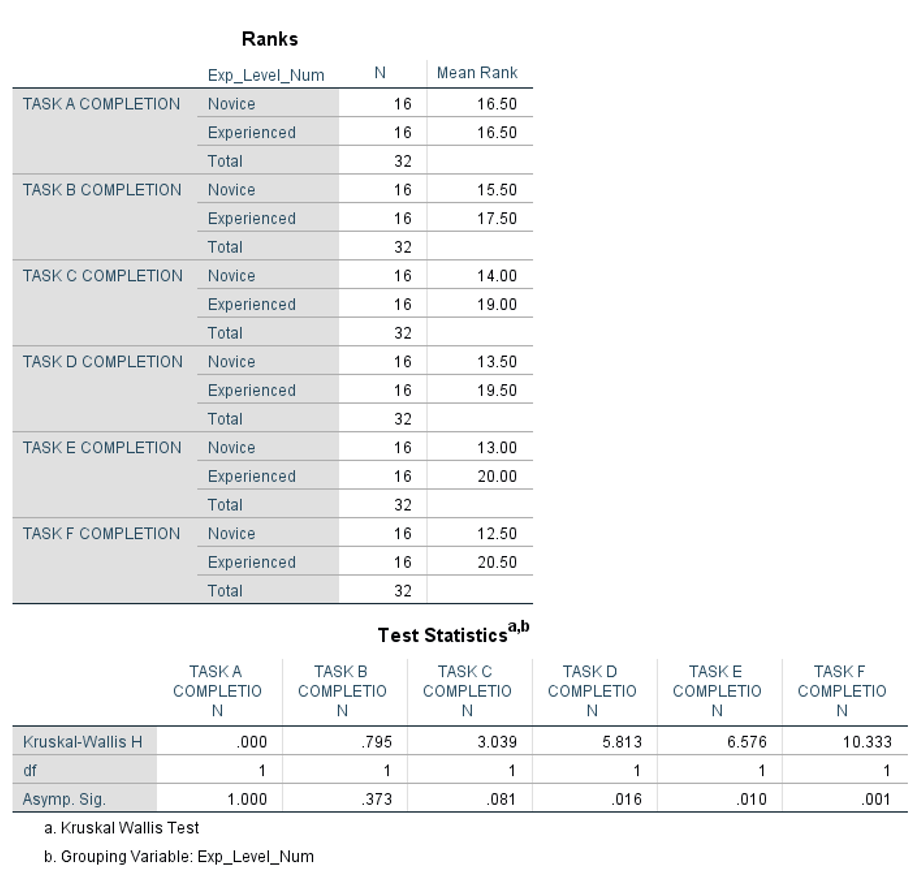
\includegraphics[width=\linewidth]{Screenshots/UXResearchDataFiles/UXTaskCompletionData/ALLTaskKWCompletionEdited.png}
\label{DescriptiveTaskCompletionALLKW}
\caption{Task Completion All Kruskal Wallis Results for all Tasks}
\end{table}

This table shows all previous Task Completion data into one table. According to the Kruskal-Wallis significance tests, Only Task F has a significant difference between that of Novice and Experienced Users, with a assumption figure of 0.01. All other tasks show no significant difference, with both Novice and Experienced users showing no difference in their completion of Task A, as all participants successfully completed the Task.

\section{Task Mouse Interactions}

\begin{table}[H]
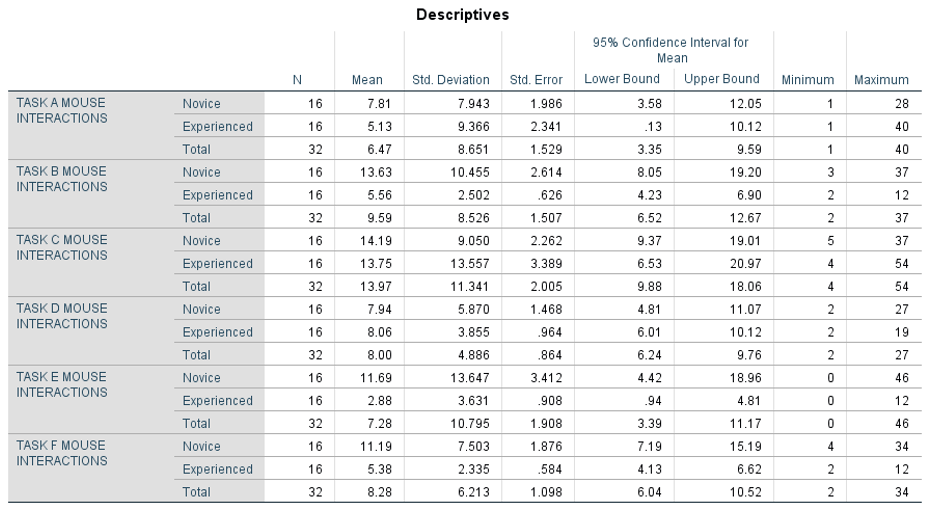
\includegraphics[width=\linewidth]{Screenshots/UXResearchDataFiles/UXTaskMouseInteractionsData/anovaDescriptivesTaskMouseInteractions.png}
\label{DescriptiveMouseInteractionsAllTasks}
\caption{Task Mouse Interactions Descriptive Statistics for Total Population}
\end{table}

As with all previous metrics Table 5.11 shows descriptive statistics taken from both Novice and Experienced participants data records of the number of Mouse Interactions made to attempt to complete each Task. As generally expected with the other other metrics collected, Novice participants overall took more mouse interactions when attempting each Task compared with their Experienced counterparts. Task C proved the most complex Task to attempt, with both Novice and Experienced participants using more mouse interactions within that Task. The maximum amount of mouse interactions made was also within Task C, with 54 clicks being recorded as the highest amount surprisingly by an Experienced participant. This participants score can be explained by the usage of the mouse provided during the experiment as the participant double clicked on each element interacted with, thus inflating their score twice as much as another participant who only single clicked on the majority of elements.

%\begin{table}[H]
%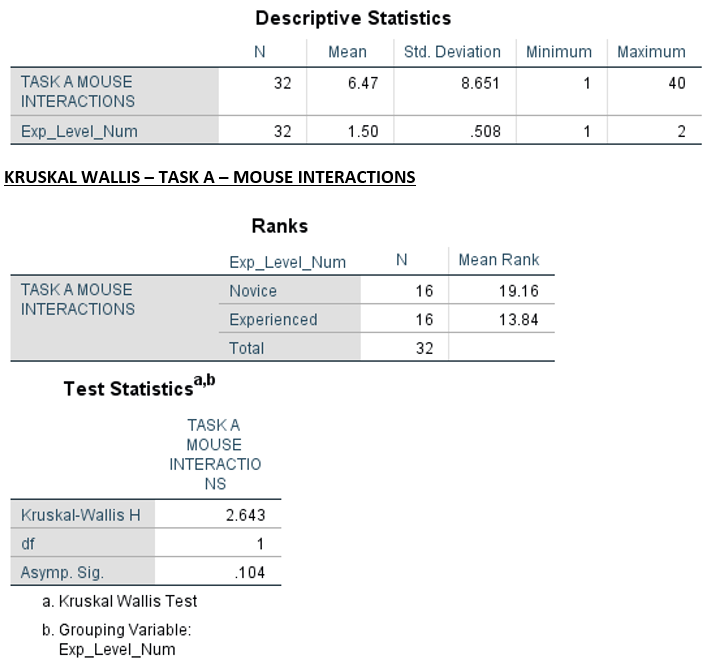
\includegraphics[width=\linewidth]{Screenshots/UXResearchDataFiles/UXTaskMouseInteractionsData/TaskAMouseInteractionsEdited.png}
%\label{TaskAMouseInteractions}
%\caption{Task A Mouse Interactions Results}
%\end{table}

%\begin{table}[H]
%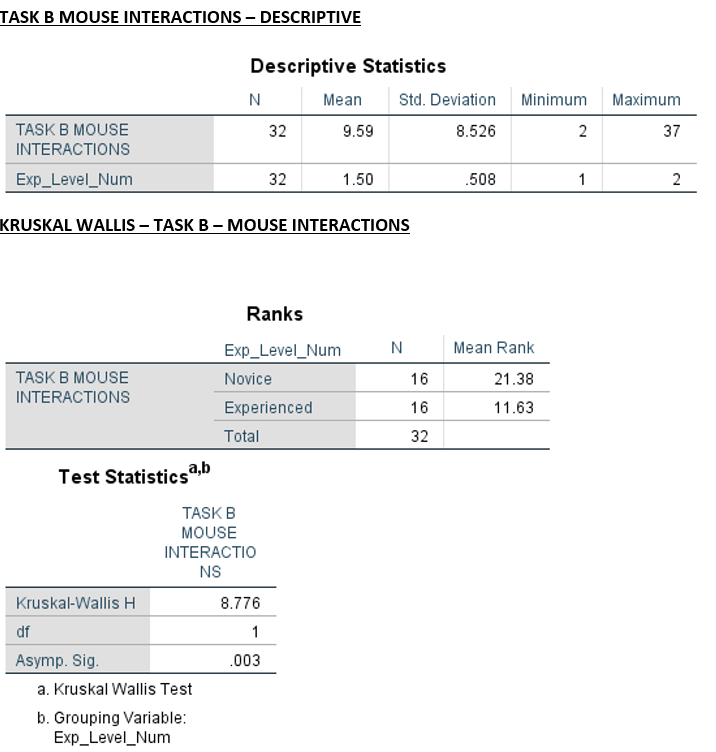
\includegraphics[width=\linewidth]{Screenshots/UXResearchDataFiles/UXTaskMouseInteractionsData/TaskBMouseInteractionsEdited.png}
%\label{TaskBMouseInteractions}
%\caption{Task B Mouse Interactions Results}
%\end{table}

%\begin{table}[H]
%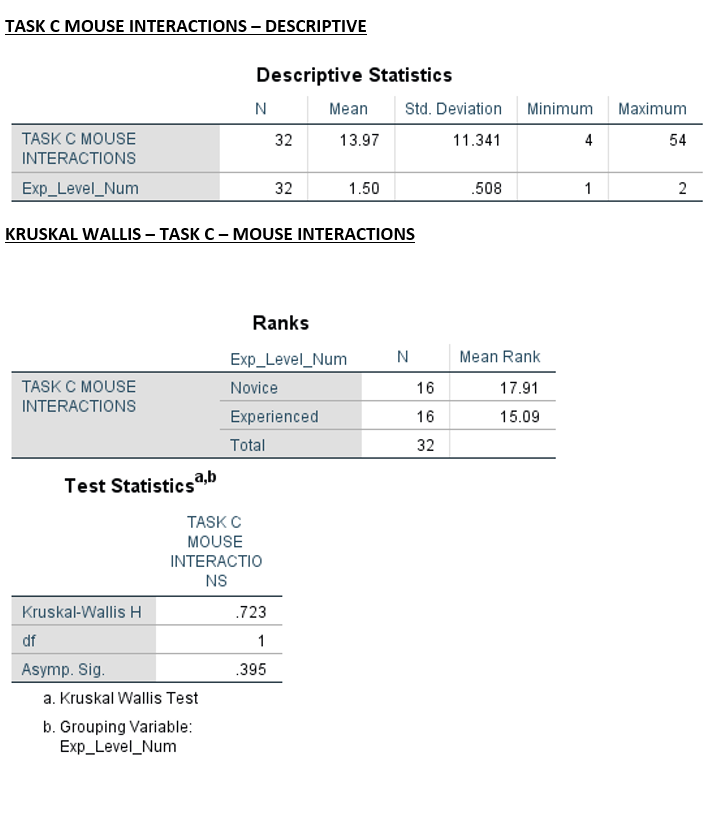
\includegraphics[width=\linewidth]{Screenshots/UXResearchDataFiles/UXTaskMouseInteractionsData/TaskCMouseInteractionsEdited.png}
%\label{TaskCMouseInteractions}
%\caption{Task C Mouse Interactions Results}
%\end{table}

%\begin{table}[H]
%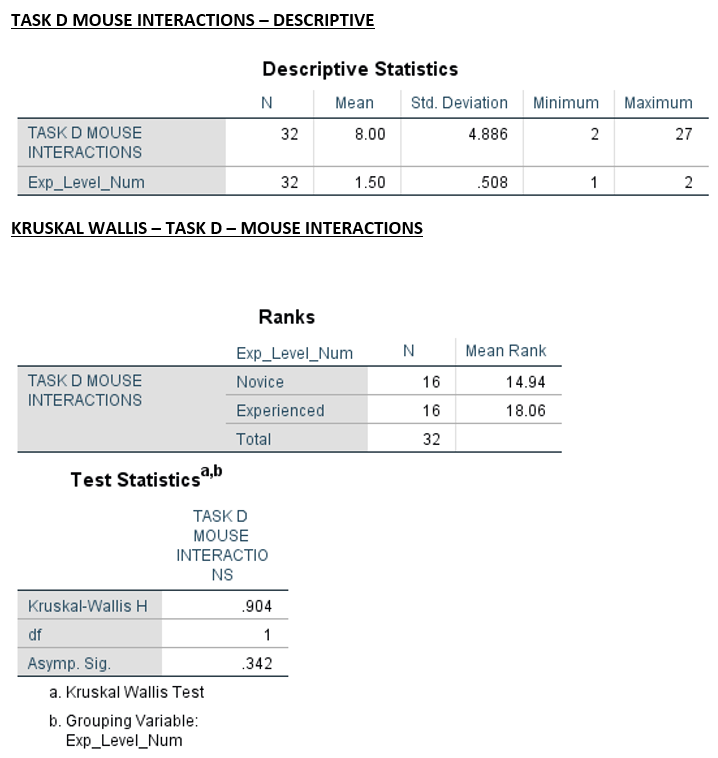
\includegraphics[width=\linewidth]{Screenshots/UXResearchDataFiles/UXTaskMouseInteractionsData/TaskDMouseInteractionsEdited.png}
%\label{TaskDMouseInteractions}
%\caption{Task D Mouse Interactions Results}
%\end{table}

%\begin{table}[H]
%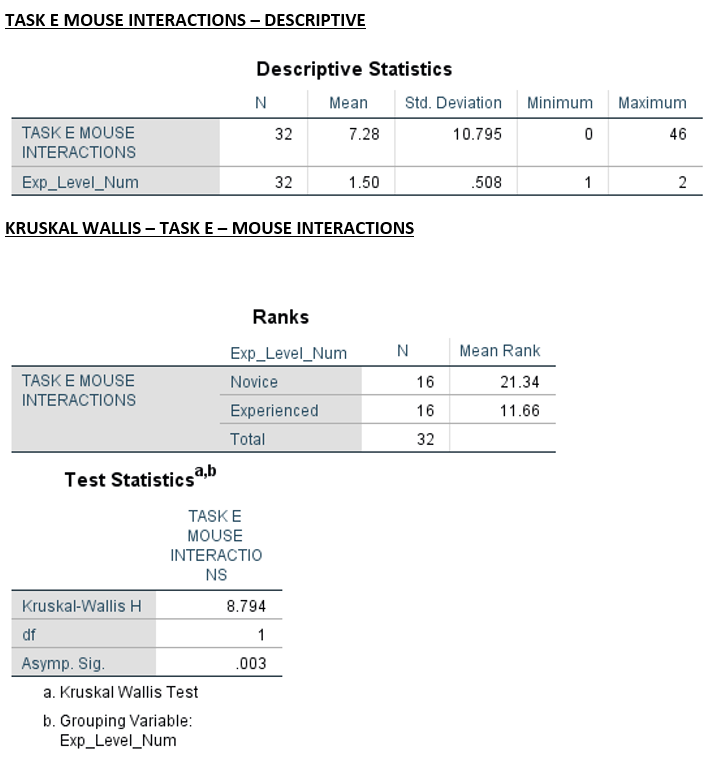
\includegraphics[width=\linewidth]{Screenshots/UXResearchDataFiles/UXTaskMouseInteractionsData/TaskEMouseInteractionsEdited.png}
%\label{TaskEMouseInteractions}
%\caption{Task E Mouse Interactions Results}
%\end{table}

%\begin{table}[H]
%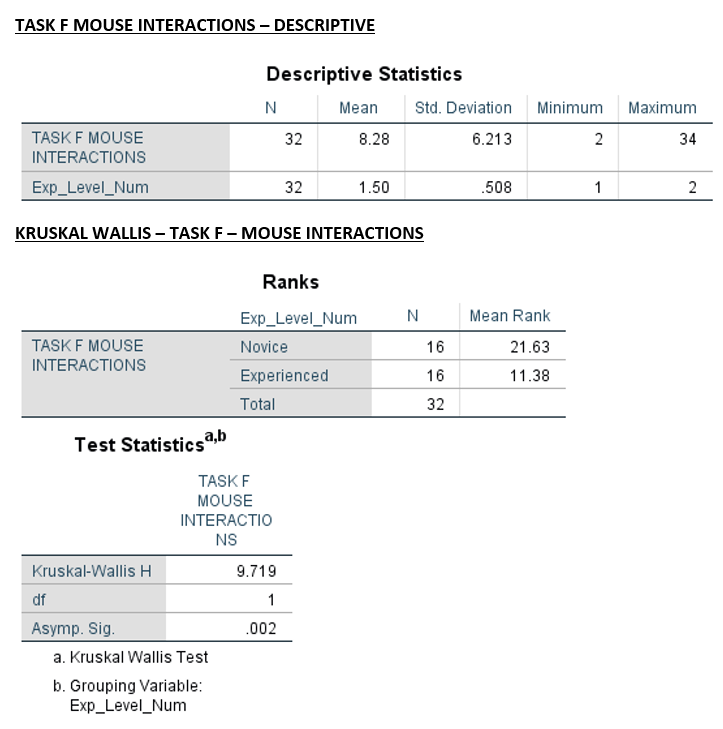
\includegraphics[width=\linewidth]{Screenshots/UXResearchDataFiles/UXTaskMouseInteractionsData/TaskFMouseInteractionsEdited.png}
%\label{TaskFMouseInteractions}
%\caption{Task F Mouse Interactions Results}
%\end{table}

\begin{table}[H]
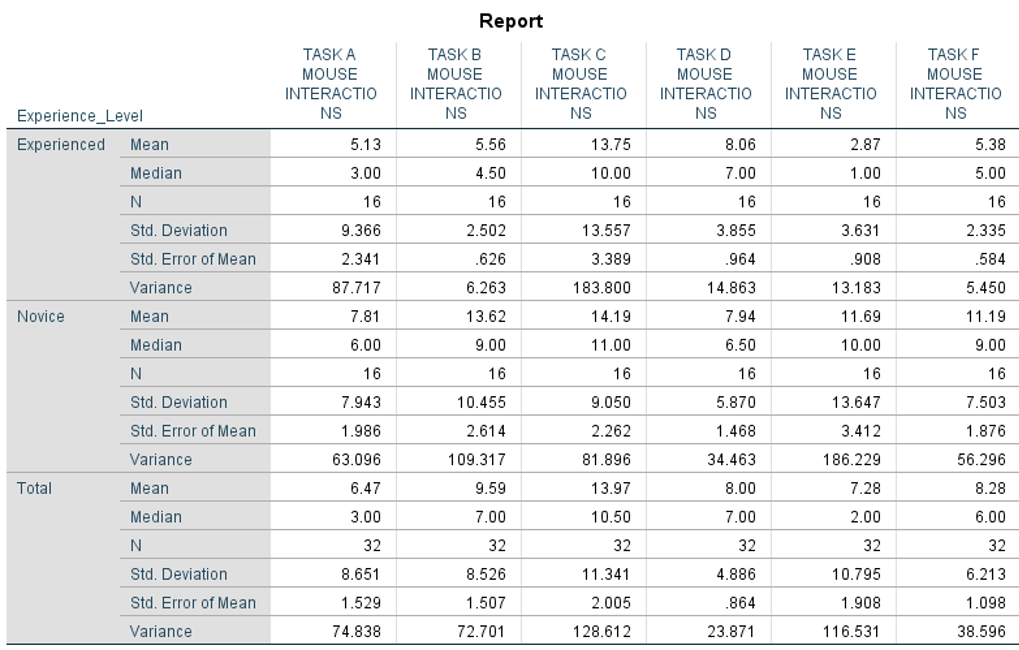
\includegraphics[width=\linewidth]{Screenshots/UXResearchDataFiles/UXTaskMouseInteractionsData/OverallDescriptiveTaskMouseInteractionsEdited.png}
\label{DescriptiveMouseInteractionsTotalPopulation}
\caption{Task Mouse Interactions Descriptive Statistics for Total Population}
\end{table}

Mouse interactions made by participants also show a notable amount of variance between Novice and Experienced participants. Novices show more variation in the amount of mouse interactions made between one another compared with internal comparison of experienced participants, with the exception of Task C, due to the inflation of one participants results, as described with Table 5.11. The highest level of variance shown within the novice data set is within Task E, with a maximum of 46 mouse interactions made by a Novice participant (See Table 5.11).

\begin{table}[H]
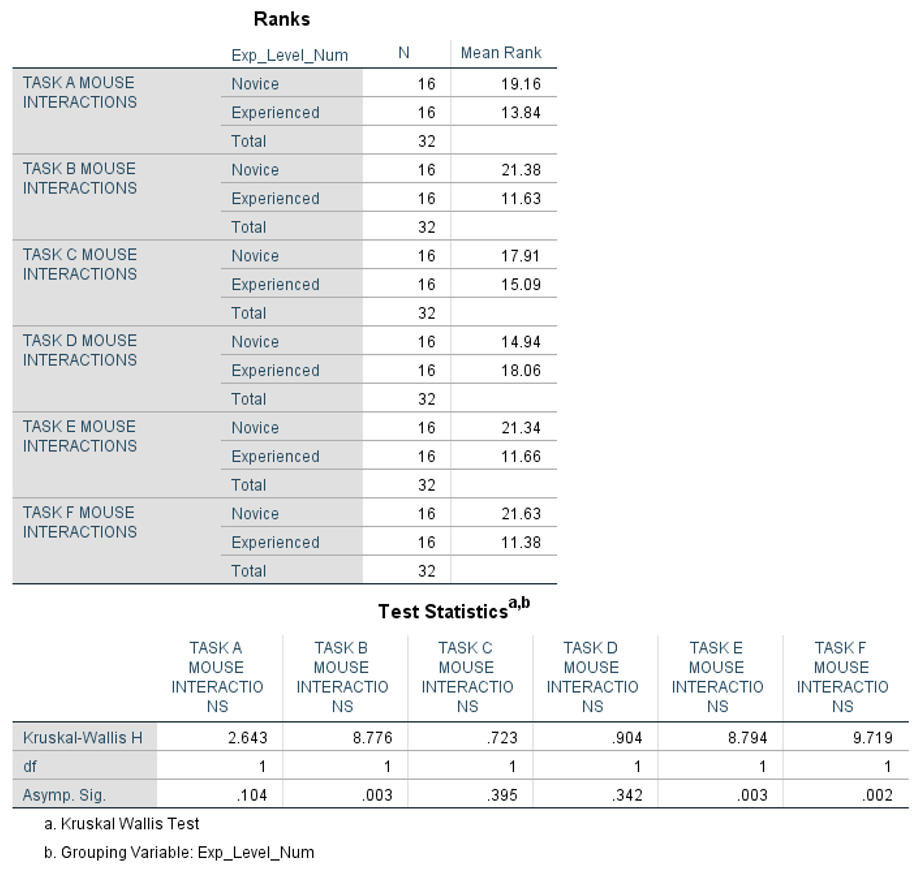
\includegraphics[width=\linewidth]{Screenshots/UXResearchDataFiles/UXTaskMouseInteractionsData/AllTasksMouseInteractionsKWEdited.png}
\label{AllMouseInteractionsKW}
\caption{Task Mouse Interactions All Kruskal Wallis Results for all Tasks}
\end{table}

Much like the previous two data metrics, this table shows all data sets for Task Mouse Interactions with the Mean rank and Kruskal-Wallis examination of the two data sets. The first Table, showing the Mean rank for the each of the Tasks shows that The majority of tasks show that Novices have a higher mean rank, with the exception of Task D. Task C is again notable for sharing a closely similar rank between the two groups. Task B, E and F show significant differences between that of Novice and Experienced groups, with these tasks all having an assumption figure of 0.05 or less. Therefore Task A, C and D do not have a significant difference between that of each experience group. This is to be expected, as has been seen with other data collected, Tasks C and D proved difficult for several of the participants regardless of experience category.
